\def\DevnagVersion{2.15}\documentclass[14 pt]{article}
\usepackage{hyperref}
\usepackage{graphics}
\usepackage{epsfig}
\usepackage{devanagari}
\textwidth 6in
\addtolength{\oddsidemargin}{-0.5in}
\textheight 9in
\addtolength{\topmargin}{-0.5in}
\setlength{\parindent}{0pt}
\setlength{\parskip}{0.5cm}
\topskip 0.0in
\pagestyle{empty}
\thispagestyle{empty}

 

\title  {\bf  COMPUTATIONAL MODELING OF LANGUAGE ACQUISITION}
\author{\large  Rishabh Nigam \\
 Shubhdeep Kochhar \\
Advisor: Dr. Amitabh Mukherjee \\
Dept. of Computer Science and Engineering \\
\{rishabhn,shubkoch, amit\} @ iitk.ac.in }
	
\begin{document}
\maketitle

{\Large \center \bf ABSTRACT  \\}

This project deals with unsupervised learning of Natural Languages. Through a Corpus of sentences which are realistic and natural, we are able to extract pattern out of them and in turn generate new sentences that were not part of original corpus. This Extraction and Generation process is applied on various Corpus of English and Hindi Language and the results are analysed. The Algorithm used for this process is called ADIOS( Automatic Distillation OF Structures).Given a corpus of strings (text or speech, DNA sequencing etc) this algorithm recursively distills a heirarchical structured patterns.For an example if we have sentences like\\
{\dn rAm Gr jAtA h\4}\\
{\dn sFtA Ev\38DwAly jAtF h\4} \\
{\dn rAm Ev\38DwAly jAtA h\4} \\
{\dn sFtA Gr jAtF h\4}\\

from these four sentences the algorithm is able to extract clusters like \{{\dn rAm{\rs ,\re}sFtA}\} and \{{\dn Gr{\rs ,\re}Ev\38DwAly}\} and able to determine pattern such as\\
 \{{\dn rAm{\rs ,\re}sFtA}\} -- \{{\dn Gr{\rs ,\re}Ev\38DwAly}\}-- \{{\dn jAtA{\rs ,\re}jAtF}\} --\{{\dn h\4}\}  \\

   

{\Large \center \bf INTRODUCTION  \\}

It is well known that the patterns that govern language production are well-formed and rule-like but it is less clear that how are they acquired and what form should such rules take.So in this project, we attempt to learn these rules, and contruct patterns in an unsupervised manner.    
We use probabilistic inference of pattern significance to clusterize similar lexicons and use recursive construction to generate more complex patterns. This way we are able to extract the patterns and rules hidden in the initial corpus of sentences and use these rules and patterns to generate more sentences. 

{\Large \center \bf THE ADIOS ALGORITHM  \\}

The algorithm which is used in this project is ADIOS(Automatic Distillation Of Structure).
The following is a small description of the MEX criterion which is used as a distillation tool for extracting the most significant patterns in the data .\\ \\
{\large \bf The MEX Criterion}
\\
In this criterion we create a pseudograph(a non-simple graph in which both loops and multiple edges are permitted) where the sentences correspond to the different paths and vertices are the unique lexicon entries, augmented by two special symbols 'begin' and 'end'. The following diagram indicates structure that we seek, namely, the bundling of paths, signifying a relatively high probability associated with a sub-structure that can be identified as a pattern.\\
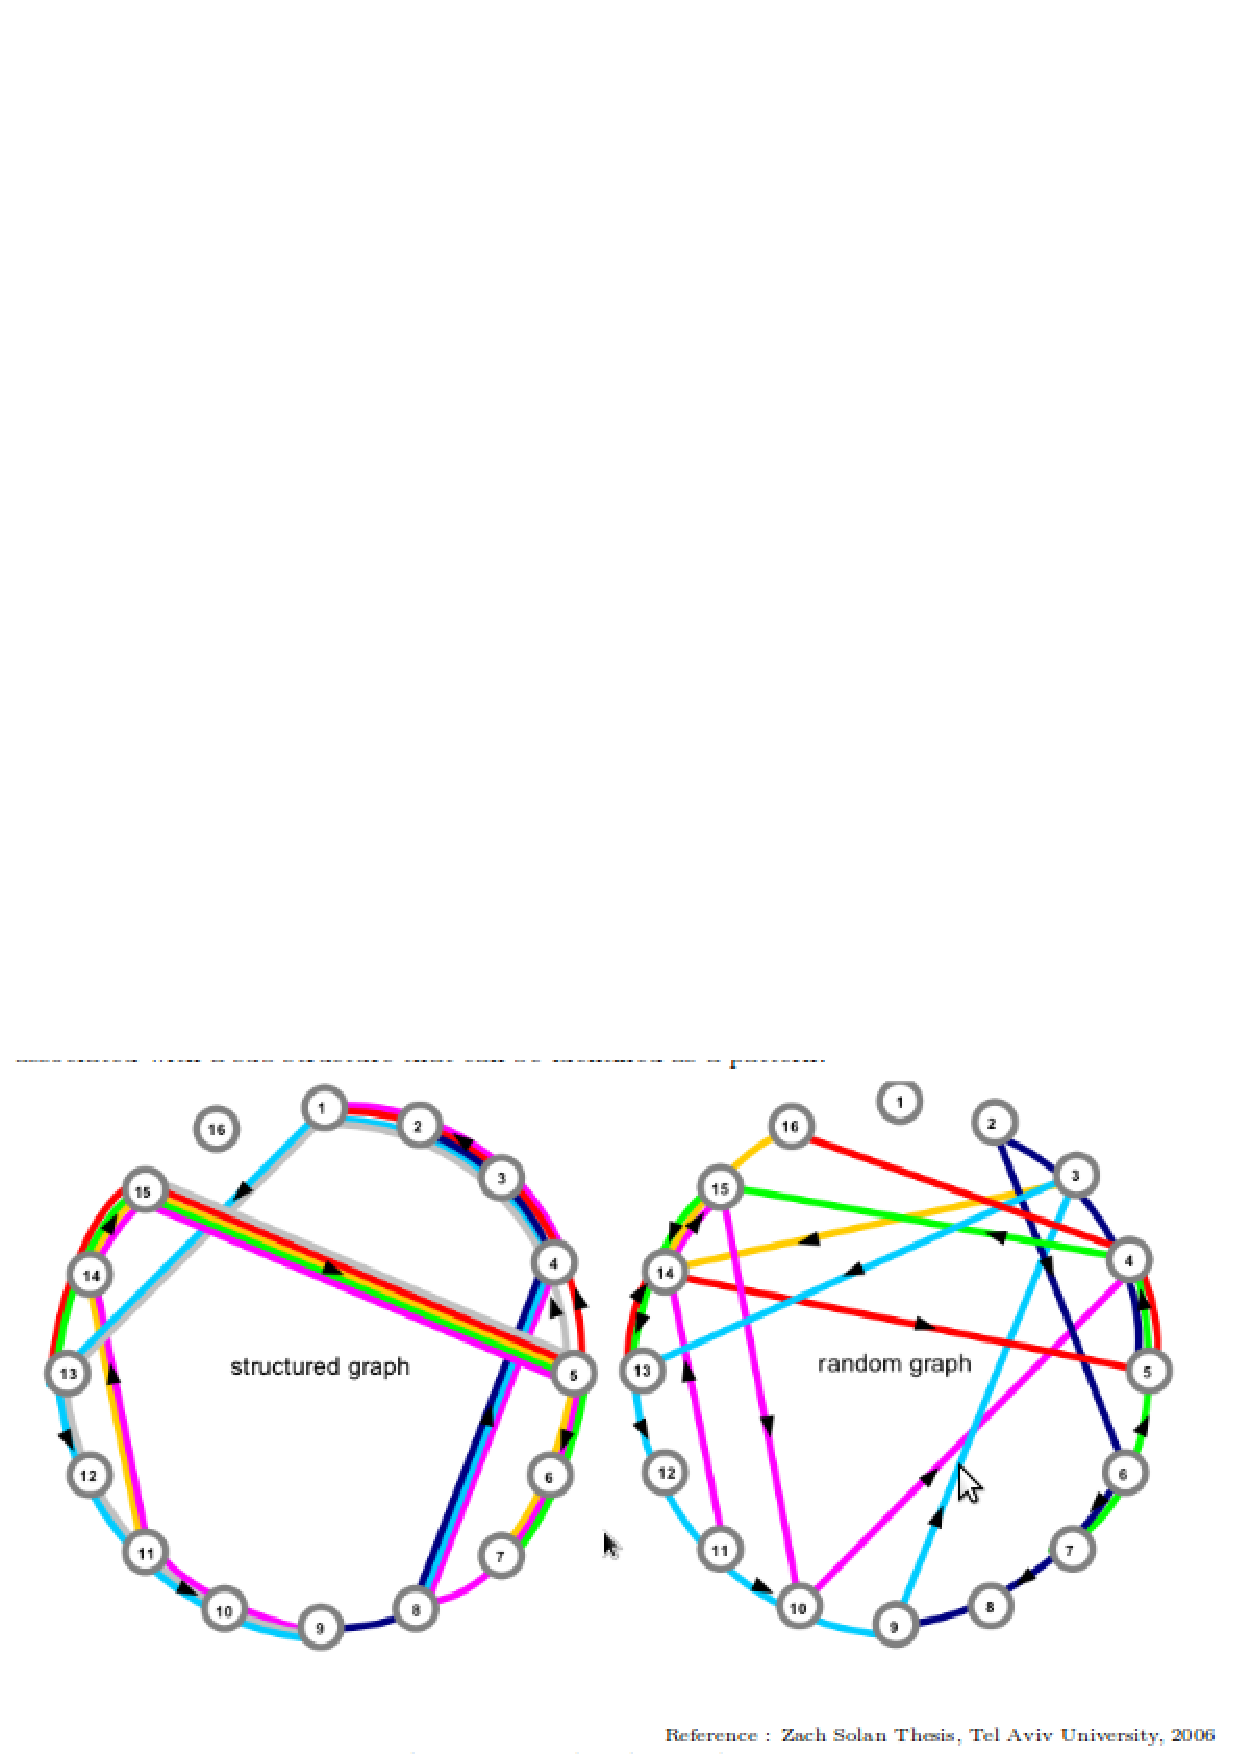
\includegraphics[width=15cm]{graph.png}
	   
\hfill {\scriptsize Reference : Zach Solan Thesis, Tel Aviv University, 2006}
\\
Firstly we define a search path S(e1 → e2 → ... → ek ) = (e1 ; ek )
Next we define two probabilty functions PR(right) and PL(left) as
\\
PR (ei ; ej ) = p(ej |ei ei+1 ei+2 ...ej−1 ) = l(ei ; ej ) / l(ei ; ej−1 )
\\
where l(ei ; ej ) is the number of occurrences of sub-paths (ei ; ej ) in the graph .
\\
Similarly proceeding from left we have
\\
PL (ej ; ei ) = p(ei |ei+1 ei+2 ...ej−1 ej ) = l(ej ; ei )/ l(ej ; ei+1 )
\\
We define decrease ratio, DR (ei ; ej ), whose value at ej is DR (ei ; ej ) = PR (ei ; ej )/PR (ei ; ej−1 )
and another decrese ratio, DL (ej ; ei ) = PL (ej ; ei )/PL (ej+1 ; ei )
\\
The algorithm calculates PL and PR from all possible starting points and this defines a matrix of the form
\\
M =  { PR(ei ; ej) i $>$j\\  
           PL(ej ; ei)    i $<$j\\
	   P(ei) 	      i = j\\
         }\\
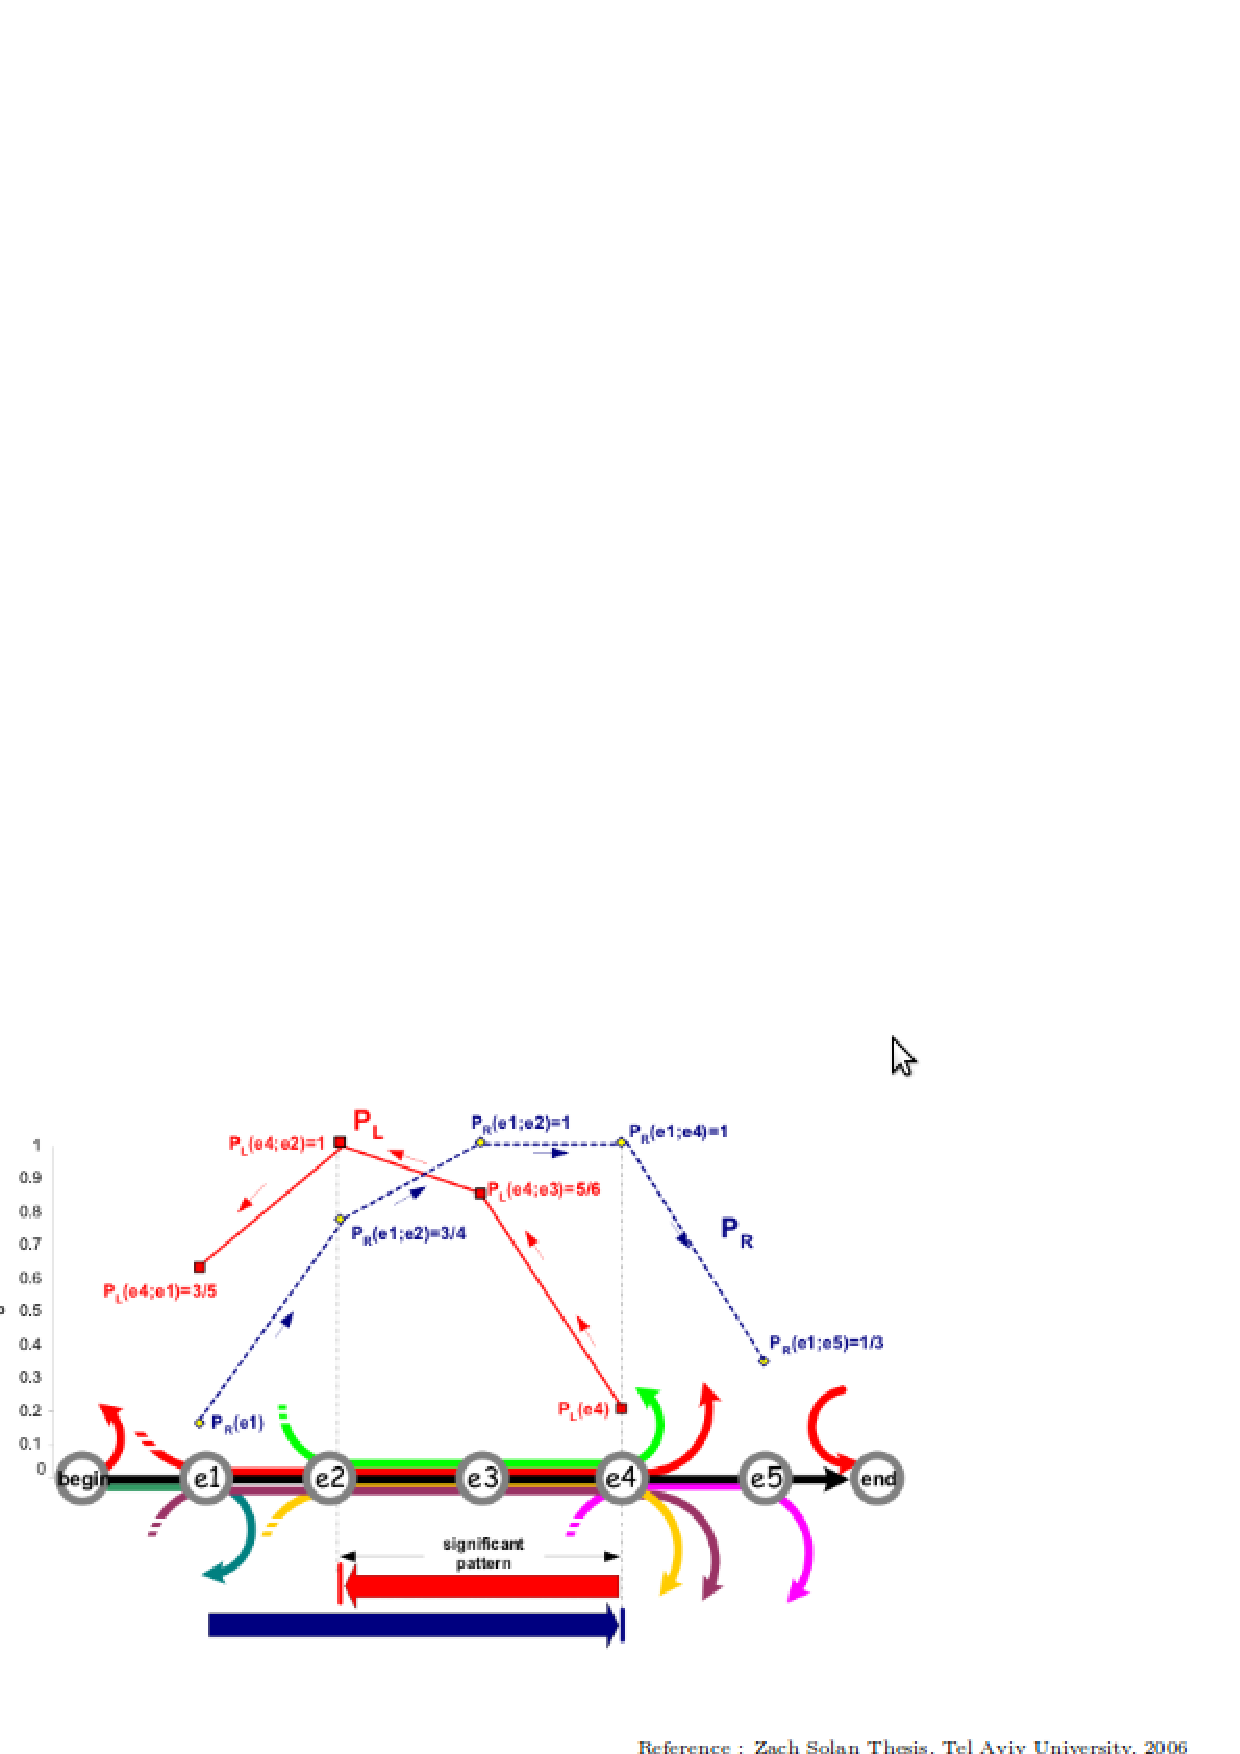
\includegraphics[width=12cm]{pattern.png}

\hfill {\scriptsize Reference : Zach Solan Thesis, Tel Aviv University, 2006}\\
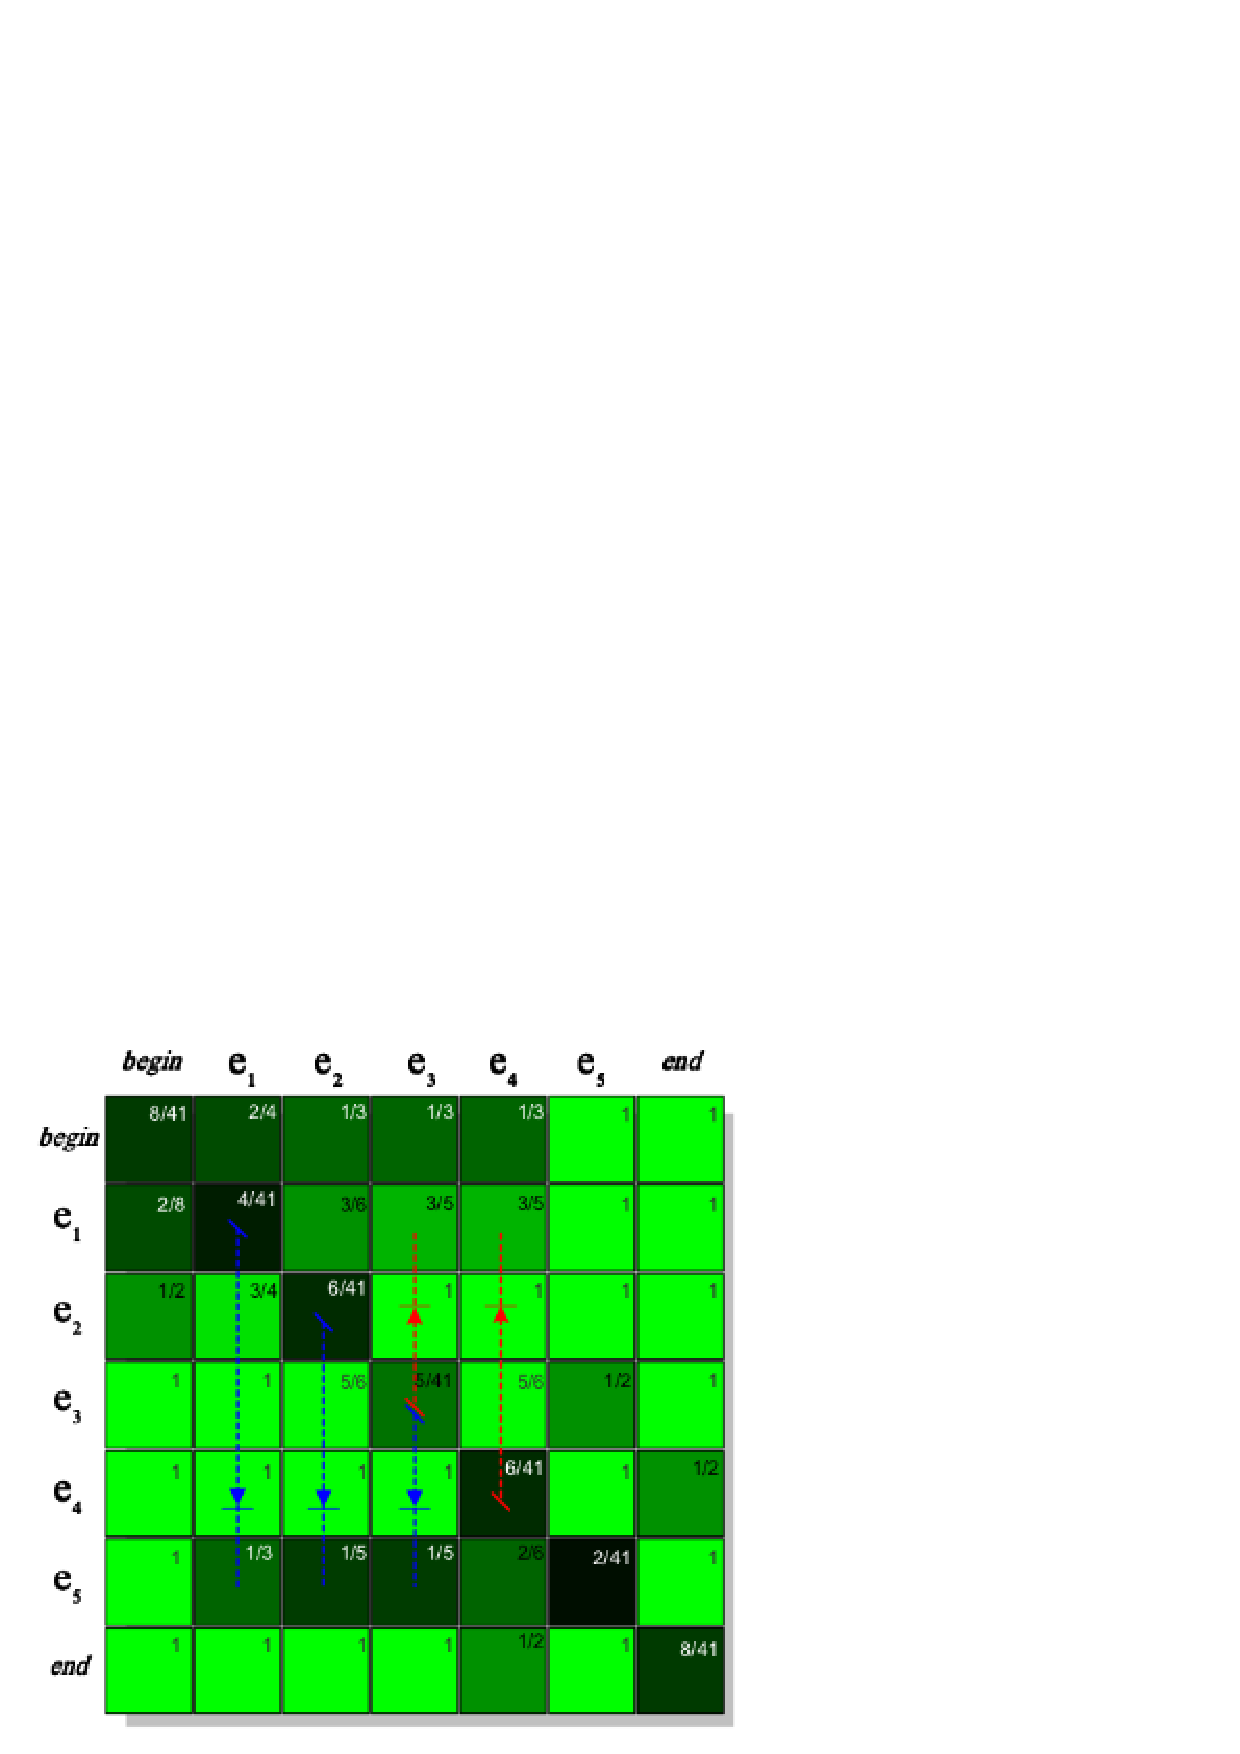
\includegraphics[width=10cm]{a.png}

\hfill {\scriptsize Reference : Zach Solan Thesis, Tel Aviv University, 2006}\\

The algorithm then identifies the leading pattern from the matrix by examining the DR and DL and is returned as the outcome of search in question.

{\large \bf The ADIOS Algorithm}
\\The algorithm works in three steps:
\begin{enumerate}
 \item INITIALIZATION: sentence loading
 \item PATTERN DISTILLATION: iterative search for significant patterns which are added to lexicons as new units
 \item GENERALIZATION: it generates more and more candidate pattern to be considered by pattern distillation
\end{enumerate} 
So an overview of ADIOS Algorithm is as follows:
\begin{enumerate}
\item {\bf Initialization} (load all sentences)
\item repeat
\item
\begin{tabbing}
 	for \= all m = 1 : N do {N is the number of paths in the graph}\\
	\> {\bf Pattern Distillation(m)} (Identifies new significant 	patterns in search-path m using the MEX criterion) 	\\
	\>	{\bf Generalization(m)} (Generate new pattern candidates for search-path (m))\\
	end for
\end{tabbing}
\item until no further significant patterns are found
\end{enumerate}


{\large \center \bf IMPLEMENTATION DETAILS\\}

The first part consisted of preprocessing of the data used, for this
we had to write a script to extract the Mother Sentences from the
CHILDES database. The CHILDES database consisted of sentences
of Mother as well as some information related to the sentences, so
we had to extract only the sentences used by the mother. \\

Then as we had most of the code for the ADIOS algorithm, we basically had
to understand and use it. For this we really had to have an
understanding of the algorithm as the code had certain parameters
which were initially not very clear. Then as the code had lots of
commands, we needed to decide on what to do first (in this the
documentation \url{http://adios.tau.ac.il/algorithm.html#Step_By_Step}
was of great help).\\


The first step was to create a Graph which the ADIOS algorithm can train on.\\

The command consisted of following script\\

{\bf  ./create\_graph.exe -f name.corpus.txt -o name} \\

The second step was to test the Algorithm on a given new unseen corpus \\

Example: \\
{\bf ./adios.exe -a train -i name.idx -g name.grp -E 0.8 -S 0.01 -o name} \\

{\bf Arguments:}\\


-a command     -$>$ select between training (train) testing (test) printing results (print) generating sentences (generate)\\

-E [0..1]      -$>$ the ETA parameter  (Default: 0.8) we used 0.8 and 0.9\\

-S [0..1]      -$>$ the patterns p-value  (Default: 0.01)\\

-C [0..1]      -$>$ the minimal coverage required from a formed Equivalence Class  (Default: 0.65)\\

-A [1..]       -$>$ The largest pattern size: All patterns with size larger than A will be treated as equal in the rewiring process.\\ 

-B {1..]       -$>$ The minimum pattern size\\

{\bf output files:}\\

name.trace.log: summary of the algorithm progress\\

name.results.txt: list of the acquired patterns and properties\\

The third step was to print and visualize the aquired patterns. We used the MATLAB codes to print the patterns obtained from the site
\url {"http://adios.tau.ac.il/algorithm.html"}

Finally we generated novel sentences from the obtained patterns through the following script

{\bf ./adios.exe -a generate -i name.idx -n 1000 -o name }\\

here -n specifies number of the sentences generated ( in this Demo version 2000 is the upper limit and the default).\\

After we understood the algorithm we implemente on the test data given with the program. Then we implemented the same on the CHILDES database to get the patterns graphs. Then we decided to run this on a Hindi database. We got the database from CFILT IIT Mumbai. Now this database again needed to be converted into suitable format, for this again we needed to do some manipulations with the file that we got. After the preprocessing stage we needed to train the grammar on the database and generate new sentences. For this we again had to
repeat the steps we used for the CHILDES database. We decided to use another set of sentences, this time doubled the number of
sentences from 2500 to 5000. We also used the algorithm on a Commentary of around 780 sentences.
\\

{\large \center \bf RESULTS\\}
For the CHILDES database, we were able to get 101 equivalence classes. For the Hindi database we were able to generate 10 equivalence classes, for the commentary we got 14 equivalence classes.\\
Some of the equivalence classes are shown in the pictures below, the complete result can be found at\\
 home.iitk.ac.in/~rishabhn/cs365/projects/\{hindi,childes,commentary\}.\{label,generate\}.txt \\

\begin{center}
{ \bf \center CHILDES\\}
\includegraphics[width=17cm]{childes1.png}\\
\newpage
 {\bf \center HINDI \\}
{\center \includegraphics[width=17cm]{hindi1.png}\\}
{\bf \center COMMENTARY \\}
\includegraphics[width=17cm]{C.png}\\
\newpage
{\bf \center SAMPLE \\ }
\includegraphics[width=17cm]{TA1.png}\\
\end{center}
{ \bf \center \large BIBLIOGRAPHY\\ }
$[$1$]$ Heider. Waterfall ,Ben Sandbank,Luca Onnis and Shimon Edelman , An empirical generative framework for computational modeling of language acquisition : Cambridge University Press 2010
http://kybele.psych.cornell.edu/~edelman/Waterfall-Sandbank-Onnis-Edelman-JCL10.pdf

$[$2$]$ Zach Solan PHD thesis, Unsupervised Learning of Natural Languages, under Professor David Horn, Professor Shimon Edelman, Professor Eytan Ruppin : Senate of Tel Aviv University 2006 [1-38]
http://horn.tau.ac.il/publications/ZachSolanThesis.pdf

$[$3$]$ CHILDES (Child Language Data Exchange System)    http://childes.psy.cmu.edu/

$[$4$]$ Dr Pushpak Bhattacharya, CFILT(Centre For Indian Language technology) IIT Bombay\\    http://www.cfilt.iitb.ac.in/Downloads.html


\end{document}